\documentclass[11pt]{amsart}
\usepackage[margin=1in]{geometry}
\usepackage{amsmath,amssymb,booktabs,array}
\usepackage{tikz}
\usepackage[colorlinks=true,linkcolor=blue,citecolor=blue,urlcolor=blue]{hyperref}
\newtheorem{theorem}{Theorem}[section]
\newtheorem{lemma}[theorem]{Lemma}
\newtheorem{proposition}[theorem]{Proposition}
\theoremstyle{definition}
\newtheorem{definition}[theorem]{Definition}
\theoremstyle{remark}
\newtheorem{remark}[theorem]{Remark}
\newcommand{\R}{\mathbb R}
\newcommand{\norm}[1]{\left\lVert #1\right\rVert}
\newcommand{\ip}[2]{\left\langle #1,#2\right\rangle}
\newcommand{\rhoSixteen}{\rho_{16}}
\newcommand{\rhoSeventeen}{\rho_{17}}
\newcommand{\rhoHex}{\sqrt6+\sqrt2}
\DeclareMathOperator{\asin}{asin}
\DeclareMathOperator{\acos}{acos}
\title[Exact circle packings for sixteen, seventeen, eighteen and twenty disks]{Exact circle packings for sixteen, seventeen, eighteen and twenty disks}
\author{Jensen Kohlmeyer}
\email{jenwin@purdue.edu}
\author{Grant Huffman}
\email{huffma97@purdue.edu}
\author{Will Howe}
\email{howew@purdue.edu}
\author{Liam Kruer}
\email{kruerl@purdue.edu}
\date{October 8, 2026; working draft}
\subjclass[2020]{52C15}
\keywords{circle packing, exact arithmetic, computer-assisted proof, interval certificates, Lean formalization}
\thanks{Prepared with AI assistance from OpenAI Codex in mathematical exploration, certificate generation and checking, manuscript preparation, and Lean development.}
\begin{document}
\begin{abstract}
We determine the smallest circular containers admitting sixteen, seventeen,
eighteen and twenty congruent unit disks, and formalize the four least-radius
theorems in Lean. A strict dilation and a maximal-boundary normalization
reduce arbitrary placements to finitely many circular orders and radial
boxes. Rational angular-cycle certificates exclude boxes away from the
attaining arrangements; equilibrium stresses give quantitative local
exclusion near critical configurations. Joint bounds on complete angular
cycles supply additional certificates for twenty disks. The eighteen-disk
optimum is $1+\sqrt2+\sqrt6$; the other three optima are specified by exact
radical closure equations and rational enclosures. Every retained
exclusion forest passes both sine- and cosine-based exact arithmetic
replays. The twenty-disk proof covers 19,796 canonical circular orders and
199,234,854 tree nodes. All four final Lean assertions have no remaining
certificate hypotheses. We state explicitly the compiled-evaluation trust
boundary of the finite \texttt{native\_decide} checks.
\end{abstract}
\maketitle

\noindent\textbf{Verification status.}
The four separate Lean least-radius theorems and their finite exclusion
certificates have compiled. Exact replay, source-binding and axiom audits
are complete for $n=16,17,18,20$. This manuscript remains a working draft
for author review.

\section{Introduction}
For $R\ge0$ write $B_R=\{x\in\R^2:\norm{x}<R\}$.
A packing of $n$ unit disks consists of $n$ images of $B_1$ under Euclidean
isometries, with pairwise disjoint images contained in $B_R$. The disks are
open, so tangencies are permitted. Let $R_n$ be the least admissible container
radius, and write $\rho_n=R_n-1$ for the corresponding center radius.

Classical arrangements and computational searches provide sharp candidates
for many values of $n$; see Graham, Lubachevsky, Nurmela and
\"Osterg\aa rd~\cite{graham} and the Packomania tables~\cite{specht}.
Ekanayake and LaFountain~\cite{ekanayake} developed a tight-partition method
and gave an independent proof for fourteen disks. Goldberg~\cite{goldberg}
described the classical candidate arrangement for twenty disks.
The present framework extends the strict-normalization and finite-certificate
approach in Huffman's fifteen-disk manuscript~\cite{huffman}.

\begin{theorem}[Sixteen and seventeen disks]\label{thm:completed}
The least container radii for sixteen and seventeen unit disks are
$1+\rhoSixteen$ and $1+\rhoSeventeen$, respectively, where the exact radical
closure roots are defined in Sections~\ref{sec:sixteen} and~\ref{sec:seventeen}.
Let
\begin{align*}
a_{16}&=4.6154255948731939855392441619919652476082,\\
a_{17}&=4.7920337483105791701491239532956924864150.
\end{align*}
Then $R_{16}\in[a_{16},a_{16}+10^{-40}]$ and
$R_{17}\in[a_{17},a_{17}+10^{-40}]$.
The lower bounds include arbitrary asymmetric arrangements.
\end{theorem}
\noindent Theorem~\ref{thm:completed} is supported by the mathematical lemmas
below and complete exact Python replays. Both least-radius assertions
have also compiled in Lean; their finite acceptance checks use the
compiled-evaluation trust boundary described in Section~\ref{sec:lean}.

\begin{theorem}[Eighteen disks]\label{thm:eighteen}
For eighteen unit disks,
\[
 R_{18}=1+\sqrt2+\sqrt6
 =4.8637033051562731469989727989155894705356\ldots.
\]
The lower bound is certified by all 4,863 normalized circular orders,
with 8,233,519 nodes accepted by two independent exact replays.
The complete least-radius assertion has also compiled in Lean.
\end{theorem}
\begin{theorem}[Twenty disks]\label{thm:twenty}
Let $\widehat q_{20}$ be the radical closure root defined in
Section~\ref{sec:twenty}. The least container radius for twenty unit disks is
$R_{20}=1+\widehat q_{20}$. In particular, with
\[
 b_{20}=5.1223207369915283214476857922008406476319,
\]
one has $R_{20}\in[b_{20},b_{20}+10^{-40}]$.
The lower bound applies to arbitrary asymmetric arrangements.
\end{theorem}

The proof separates discovery from acceptance. Floating point arithmetic may
choose a subdivision or propose a witness, but every accepted leaf is a
finite exact inequality or an application of a proved local theorem. A
complete certificate includes every required order, every child of every
split, and no unresolved leaf. A feasible candidate alone gives an upper
bound and does not establish optimality.

\section{Centers, dilation, and boundary normalization}\label{sec:normalization}
\begin{lemma}\label{lem:centers}
Open unit disks with centers $x,y$ are disjoint exactly when $\norm{x-y}\ge2$.
The disk with center $x$ lies in $B_R$ exactly when $\norm{x}+1\le R$.
\end{lemma}
\begin{proof}
If $\norm{x-y}<2$, their midpoint belongs to both disks. A common point
conversely contradicts the triangle inequality when $\norm{x-y}\ge2$.
The containment inequality is sufficient by the triangle inequality. If it
fails, points less than unit distance from $x$ in the outward radial direction
have norm exceeding $R$; at $x=0$ any unit direction suffices.
\end{proof}

\begin{lemma}[Strict dilation]\label{lem:strict}
If an $n\ge2$ disk packing fits in radius $R<1+q$, then there are $n$ centers
$x_i$ with $\norm{x_i}\le q$ and $\norm{x_i-x_j}>2$ for $i\ne j$.
\end{lemma}
\begin{proof}
Their original center radius $r=R-1$ is positive by pair separation.
Multiplication by $q/r>1$ gives the assertion.
\end{proof}

\begin{lemma}[Maximal-boundary normalization]\label{lem:push}
Suppose strictly separated centers exist in the closed disk of radius $q>2$.
They can be chosen so that every center radius is either $q$ or less than
$D(q)=q-4/q$, and at least one radius equals $q$.
\end{lemma}
\begin{proof}
Choose a strict configuration with the greatest integer number of boundary
centers. The possible counts form a nonempty finite set, so no compactness
assumption about strict packings is needed. If there is no boundary center,
replace a farthest center $sv$, $\norm v=1$, by $qv$. For any other center
with $\norm z\le s<q$,
\[
\norm{qv-z}^2-\norm{sv-z}^2
 =(q-s)(q+s-2\ip vz)>0.
\]
This contradicts maximality. If a nonboundary center has radius at least
$D(q)$, choose a farthest such center $sv$. Its distances to other interior
centers increase by the same identity. For a boundary center $z$,
\[
\norm{qv-z}^2-4
 =\frac qs(\norm{sv-z}^2-4)
  +\frac qs(q-s)(s-D(q))>0.
\]
The replacement again increases the boundary count. Only the final
replacement is asserted feasible; a continuous radial motion is not required.
\end{proof}

\section{Exact feasible constructions}
\subsection{Sixteen disks}\label{sec:sixteen}
For $q$ in the interval defining $\rhoSixteen$ put
\[
h=1-2/q^2,\qquad k=2\sqrt{q^2-1}/q^2,\qquad
U(x,y)=(hx-ky,kx+hy).
\]
Let $Q_0=(0,-q)$ and $Q_{j+1}=UQ_j$ for $0\le j<5$, writing
$Q_j=(X_j,Y_j)$. Define
\begin{align*}
a&=Y_1+\sqrt{4-(X_1-1)^2}, & c&=Y_5-\sqrt{4-X_5^2},\\
t&=c-a, & u&=\sqrt{\frac{15-t^2}{4(1+t^2)}},\\
A&=(1,a), & B&=(\tfrac12+tu,\tfrac12(a+c)+u),\qquad C=(0,c).
\end{align*}
With $m(x,y)=(-x,y)$, the centers are
\[
\{Q_0,\ldots,Q_5,m(Q_1),\ldots,m(Q_5),A,m(A),B,m(B),C\}.
\]
The exact definition of $\rhoSixteen$ is the unique root in the center-radius
interval obtained from Theorem~\ref{thm:completed} by subtracting one, of
\[
 F_{16}(q)=\norm{B-Q_3}^2-4=0.
\]
All radicands are positive there. Exact interval differentiation proves
$13.4453214223675<F'_{16}(q)<13.4453214223676$ and opposite endpoint signs;
continuity and the mean value theorem prove existence and uniqueness.

The rotation identities $h^2+k^2=1$ and $2q^2(1-h)=4$ prove the ten outer
chain contacts. The five inner centers form the equilateral cycle
$A,B,C,m(B),m(A),A$, since
\[
\norm{B-A}^2=\norm{B-C}^2=(1+t^2)(\tfrac14+u^2)=4.
\]
The definitions of $a,c$ and the closure equation give six inner--outer
contacts. Thus there are twenty-one disk contacts and eleven wall contacts.
The remaining ninety-nine pair distances are strictly greater than two;
their certified squared minimum exceeds $4.15861112360514$.
All five interior norms are strictly less than $q$, proving attainment.
The left panel of Figure~\ref{fig:sixteen-seventeen} shows the construction.

\subsection{Seventeen disks}\label{sec:seventeen}
Use the same $h,k,U$ and let $\sigma=\sqrt3$. Define
\begin{align*}
P&=(1,-\sqrt{q^2-1}), & Q&=UP,\\
A&=(0,P_y+\sigma), & B&=(Q_x-1,Q_y+\sigma),\\
T&=(0,B_y+\sqrt{4-B_x^2}).
\end{align*}
Write $b^2=\norm B^2$, $a=(b^2+q^2-4)/(2b^2)$,
$u=\sqrt{q^2/b^2-a^2}$, and put
\[
 W=(aB_x-uB_y,aB_y+uB_x),\qquad V=UW.
\]
For $d_x=V_x$, $d_y=V_y-T_y$, $\ell=d_x^2+d_y^2$ and
$v=\sqrt{4/\ell-1/4}$, define
\begin{align*}
C&=(d_x/2-d_yv,(V_y+T_y)/2+d_xv),\\
D&=(0,C_y+\sqrt{4-C_x^2}),\\
E&=((C_x+\sigma(D_y-C_y))/2,(C_y+D_y+\sigma C_x)/2).
\end{align*}
The seventeen centers are the seven reflected pairs
$P,Q,B,W,V,C,E$ and the three axis centers $A,T,D$.
The exact $\rhoSeventeen$ is the unique root in its stated center-radius
interval of
\[
 F_{17}(q)=\norm E^2-q^2=0.
\]
Positive radicands, opposite endpoint signs, and $F'_{17}(q)<-38.3663465154$
are checked by exact intervals. The construction gives twenty-five disk
contacts and ten wall contacts; the other 111 squared distances exceed
$4.14125268181745$. The seven interior centers lie strictly inside $q$.
The two axis centers $T,D$ have equal polar angle, and both possible orders
are retained in the local and global arguments.
The right panel of Figure~\ref{fig:sixteen-seventeen} shows the construction.

% BEGIN CONSTRUCTION DIAGRAMS 16 17
\begin{figure}[htbp]
\centering
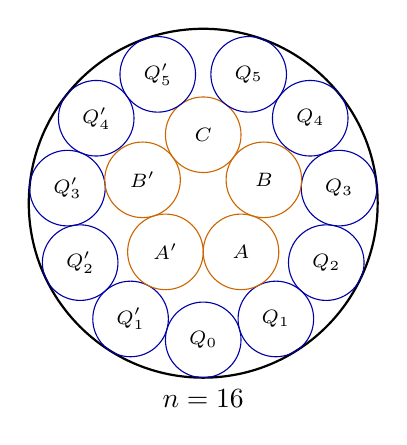
\begin{tikzpicture}[scale=.48,every node/.style={font=\scriptsize}]
\draw[thick] (0,0) circle (4.615425594873);
\draw[blue!65!black] (0.000000000000,-3.615425594873) circle (1);
\node at (0.000000000000,-3.615425594873) {$Q_0$};
\draw[blue!65!black] (-1.921974535034,-3.062240375729) circle (1);
\node at (-1.921974535034,-3.062240375729) {$Q_1'$};
\draw[blue!65!black] (1.921974535034,-3.062240375729) circle (1);
\node at (1.921974535034,-3.062240375729) {$Q_1$};
\draw[blue!65!black] (-3.255798172503,-1.571967077260) circle (1);
\node at (-3.255798172503,-1.571967077260) {$Q_2'$};
\draw[blue!65!black] (3.255798172503,-1.571967077260) circle (1);
\node at (3.255798172503,-1.571967077260) {$Q_2$};
\draw[orange!80!black] (-1.000000000000,-1.287426876584) circle (1);
\node at (-1.000000000000,-1.287426876584) {$A'$};
\draw[orange!80!black] (1.000000000000,-1.287426876584) circle (1);
\node at (1.000000000000,-1.287426876584) {$A$};
\draw[blue!65!black] (-3.593302356959,0.399349976254) circle (1);
\node at (-3.593302356959,0.399349976254) {$Q_3'$};
\draw[blue!65!black] (3.593302356959,0.399349976254) circle (1);
\node at (3.593302356959,0.399349976254) {$Q_3$};
\draw[orange!80!black] (-1.605373248664,0.618753395532) circle (1);
\node at (-1.605373248664,0.618753395532) {$B'$};
\draw[orange!80!black] (1.605373248664,0.618753395532) circle (1);
\node at (1.605373248664,0.618753395532) {$B$};
\draw[orange!80!black] (0.000000000000,1.811555446366) circle (1);
\node at (0.000000000000,1.811555446366) {$C$};
\draw[blue!65!black] (-2.831206121147,2.248460391389) circle (1);
\node at (-2.831206121147,2.248460391389) {$Q_4'$};
\draw[blue!65!black] (2.831206121147,2.248460391389) circle (1);
\node at (2.831206121147,2.248460391389) {$Q_4$};
\draw[blue!65!black] (-1.202721496211,3.409510703109) circle (1);
\node at (-1.202721496211,3.409510703109) {$Q_5'$};
\draw[blue!65!black] (1.202721496211,3.409510703109) circle (1);
\node at (1.202721496211,3.409510703109) {$Q_5$};
\node[font=\normalsize] at (0,-5.165425594873) {$n=16$};
\end{tikzpicture}
\hspace{1cm}
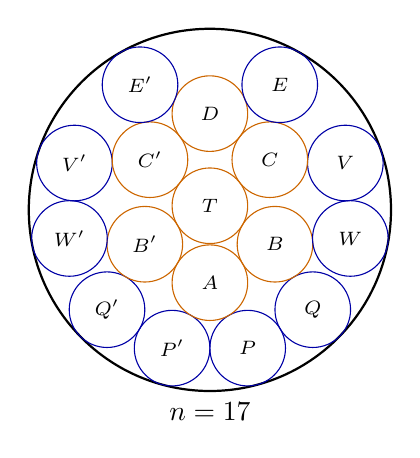
\begin{tikzpicture}[scale=.48,every node/.style={font=\scriptsize}]
\draw[thick] (0,0) circle (4.792033748311);
\draw[blue!65!black] (-1.000000000000,-3.657802611996) circle (1);
\node at (-1.000000000000,-3.657802611996) {$P'$};
\draw[blue!65!black] (1.000000000000,-3.657802611996) circle (1);
\node at (1.000000000000,-3.657802611996) {$P$};
\draw[blue!65!black] (-2.721826596828,-2.640299211287) circle (1);
\node at (-2.721826596828,-2.640299211287) {$Q'$};
\draw[blue!65!black] (2.721826596828,-2.640299211287) circle (1);
\node at (2.721826596828,-2.640299211287) {$Q$};
\draw[orange!80!black] (0.000000000000,-1.925751804427) circle (1);
\node at (0.000000000000,-1.925751804427) {$A$};
\draw[orange!80!black] (-1.721826596828,-0.908248403718) circle (1);
\node at (-1.721826596828,-0.908248403718) {$B'$};
\draw[orange!80!black] (1.721826596828,-0.908248403718) circle (1);
\node at (1.721826596828,-0.908248403718) {$B$};
\draw[blue!65!black] (-3.715992219016,-0.755593658349) circle (1);
\node at (-3.715992219016,-0.755593658349) {$W'$};
\draw[blue!65!black] (3.715992219016,-0.755593658349) circle (1);
\node at (3.715992219016,-0.755593658349) {$W$};
\draw[orange!80!black] (0.000000000000,0.109254996991) circle (1);
\node at (0.000000000000,0.109254996991) {$T$};
\draw[blue!65!black] (-3.583556676617,1.240016731259) circle (1);
\node at (-3.583556676617,1.240016731259) {$V'$};
\draw[blue!65!black] (3.583556676617,1.240016731259) circle (1);
\node at (3.583556676617,1.240016731259) {$V$};
\draw[orange!80!black] (-1.585507818754,1.328338651491) circle (1);
\node at (-1.585507818754,1.328338651491) {$C'$};
\draw[orange!80!black] (1.585507818754,1.328338651491) circle (1);
\node at (1.585507818754,1.328338651491) {$C$};
\draw[orange!80!black] (0.000000000000,2.547422305991) circle (1);
\node at (0.000000000000,2.547422305991) {$D$};
\draw[blue!65!black] (-1.848511323513,3.310970527681) circle (1);
\node at (-1.848511323513,3.310970527681) {$E'$};
\draw[blue!65!black] (1.848511323513,3.310970527681) circle (1);
\node at (1.848511323513,3.310970527681) {$E$};
\node[font=\normalsize] at (0,-5.342033748311) {$n=17$};
\end{tikzpicture}
\caption{The attaining constructions for sixteen and seventeen unit disks.
Boundary disks are blue and interior disks are orange. Center labels agree
with the radical formulas; a prime denotes reflection in the vertical axis.
The displayed coordinates are rounded from the certified enclosures.}
\label{fig:sixteen-seventeen}
\end{figure}
% END CONSTRUCTION DIAGRAMS 16 17

\subsection{Eighteen disks}\label{sec:hexagonal}
Put $s=\sqrt3$ and $q=\rhoHex$, so $q^2=8+4s$. Let
\begin{align*}
\mathcal O={}&\{(\pm(2+s),\pm1),(\pm1,\pm(2+s)),
                   (\pm(1+s),\pm(1+s))\},\\
\mathcal I={}&\{(\pm2,0),(\pm1,\pm s)\},
\end{align*}
where signs are chosen independently. These sets contain twelve and six
points, respectively. The eighteen-disk construction is $\mathcal O\cup
\mathcal I$.
All outer squared norms are $q^2$, and inner squared norms are four.
Pair differences lie in $\mathbb Q(s)^2$, so their squared lengths reduce
using $s^2=3$. Exact finite enumeration verifies thirty disk contacts.
Every noncontact squared distance is at least eight. Hence the packing
fits in radius $1+q$.

\begin{figure}[ht]
\centering
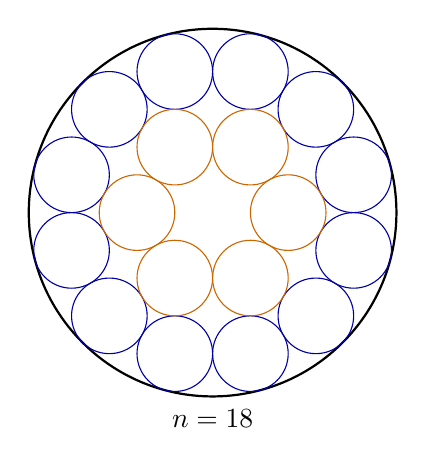
\begin{tikzpicture}[scale=.48]
\def\s{1.7320508075688772}
\def\q{3.8637033051562731}
\draw[thick] (0,0) circle ({1+\q});
\foreach \a in {15,45,...,345}{\draw[blue!65!black] ({\q*cos(\a)},{\q*sin(\a)}) circle (1);}
\foreach \a in {0,60,...,300}{\draw[orange!80!black] ({2*cos(\a)},{2*sin(\a)}) circle (1);}
\node at (0,-5.45) {$n=18$};
\end{tikzpicture}
\caption{The attaining eighteen-disk arrangement.
The figure illustrates the upper bound; the global lower bound requires the
separate exclusion argument.}
\label{fig:hexagonal}
\end{figure}

\subsection{Twenty disks}\label{sec:twenty}
Let $q$ lie in the rational interval $[a_{20},a_{20}+10^{-40}]$, where
\[
 a_{20}=4.1223207369915283214476857922008406476319.
\]
Use the rotation $U$ defined in Section~\ref{sec:sixteen}, and put
$Q_0=(1,-\sqrt{q^2-1})$, $Q_j=U^jQ_0$ for $0\le j\le5$.
For distinct points $p,z$ with $\norm{z-p}<4$ define
\[
 L(p,z)=\frac{p+z}{2}
       +\sqrt{\frac4{\norm{z-p}^2}-\frac14}\,J(z-p),
 \qquad J(x,y)=(-y,x).
\]
The two orthogonal summands give
$\norm{L(p,z)-p}^2=\norm{L(p,z)-z}^2=4$. Set
\[
 A=(1,Q_{0,y}+2),\quad B=L(A,Q_2),\quad C=L(B,Q_4),
 \quad D=(0,C_y+\sqrt{4-C_x^2}).
\]
The twenty centers are $Q_j,m(Q_j)$ for $0\le j\le5$, the pairs
$A,m(A),B,m(B),C,m(C)$, and the two axis points $D,0$.
Choose any root $\widehat q_{20}$ in the stated interval of
\[
 F_{20}(q)=\norm{D-Q_5}^2-4=0.
\]
Exact interval bounds give a negative left endpoint value and a positive
right endpoint value. All denominators and radicands remain positive,
so continuity and the intermediate value theorem give such a root.
Rotation, reflection, the two intersection identities and the closure
equation prove twelve wall contacts and twenty-six disk contacts.
All 164 other squared distances exceed $4.23462213177290$, and all eight
interior centers lie inside the center circle. Thus
$R_{20}\le1+\widehat q_{20}$. The global exclusion in
Section~\ref{sec:assembly} gives the matching lower bound.
The root-existence and feasible-packing assertions have compiled in Lean,
including all contact identities and noncontact interval checks.

\begin{figure}[ht]
\centering
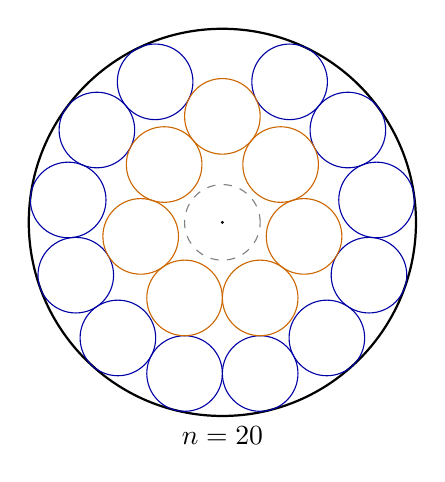
\begin{tikzpicture}[scale=.48]
\draw[thick] (0,0) circle (5.12232073699);
\draw[blue!65!black] (-1.00000000000,-3.99919095051) circle (1);
\draw[blue!65!black] (1.00000000000,-3.99919095051) circle (1);
\draw[blue!65!black] (-2.76461627396,-3.05784648345) circle (1);
\draw[blue!65!black] (2.76461627396,-3.05784648345) circle (1);
\draw[blue!65!black] (-3.87848686831,-1.39673471748) circle (1);
\draw[blue!65!black] (3.87848686831,-1.39673471748) circle (1);
\draw[blue!65!black] (-4.07942477221,0.59314567058) circle (1);
\draw[blue!65!black] (4.07942477221,0.59314567058) circle (1);
\draw[blue!65!black] (-3.32013247315,2.44340922062) circle (1);
\draw[blue!65!black] (3.32013247315,2.44340922062) circle (1);
\draw[blue!65!black] (-1.77933502163,3.71853400407) circle (1);
\draw[blue!65!black] (1.77933502163,3.71853400407) circle (1);
\draw[orange!80!black] (-1.00000000000,-1.99919095051) circle (1);
\draw[orange!80!black] (1.00000000000,-1.99919095051) circle (1);
\draw[orange!80!black] (-2.16152453645,-0.37104453473) circle (1);
\draw[orange!80!black] (2.16152453645,-0.37104453473) circle (1);
\draw[orange!80!black] (-1.54079745152,1.53019134912) circle (1);
\draw[orange!80!black] (1.54079745152,1.53019134912) circle (1);
\draw[orange!80!black] (0.00000000000,2.80531613258) circle (1);
\draw[gray,dashed] (0,0) circle (1);
\fill (0,0) circle (.04);
\node at (0,-5.65) {$n=20$};
\end{tikzpicture}
\caption{The twenty-disk construction. The dashed disk at the origin has
no contacts and is omitted from the stressed nineteen-center core.
The displayed decimal coordinates illustrate the exact radical construction.}
\label{fig:twenty}
\end{figure}

\section{Finite orders and exact angular certificates}\label{sec:certificates}
Sort centers weakly by polar angle, assigning an arbitrary angle to a possible
origin and either order to equal angles. Encode boundary centers by $0$ and
interior centers by $1$. Cyclic changes of starting point and reversal are
realized by relabelling and reflection; they do not assume symmetry of the
hypothetical packing. The root boxes are
$[q_{\rm lo},q_{\rm hi}]$ for boundary radii and
$[0,q_{\rm hi}-4/q_{\rm hi}]$ for interior radii.
Strict separation implies $r_i+r_j>2$. Thus raising an interior lower
endpoint to $2-U_j$, where $U_j$ bounds another interior radius, preserves
all feasible vectors. Every split retains both closed midpoint halves.

\begin{lemma}[Four-corner angular bound]\label{lem:corner}
Let $I,J$ be intervals of nonnegative radii, $0<t<\pi$, and $C_-(t)\le\cos t$.
If at every corner $(r,s)$ of $I\times J$,
\[
 r^2+s^2-2rsC_-(t)\le4,
\]
then pair distance greater than two forces the minor angle to exceed $t$.
\end{lemma}
\begin{proof}
The displayed expression is separately convex in $r,s$, hence attains its
maximum at a corner. It bounds the squared chord at angle $t$ from above.
Chord length is nondecreasing with the minor angle. At zero radius the same
test remains valid and requires no division by the radius.
\end{proof}

For an edge $i\to j$ in weakly sorted order define its directed gap as
$\alpha_j-\alpha_i+2\pi$ if $j<i$, and $\alpha_j-\alpha_i$ otherwise.
These gaps are nonnegative, including ties. On a directed cycle they sum to
$2\pi w$, where $w$ is the number of descending-index edges. A cycle whose
certified lower angles sum to more than $2\pi_{\rm hi}w$ excludes the whole box.

One checker uses the exact cosine polynomial
$\sum_{k=0}^{21}(-1)^k t^{2k}/(2k)!$, ending with its negative degree-42 term.
Its alternating remainder is positive for $t\le\pi$.
The independent checker bounds sine from above by a positive-ending Taylor
polynomial at $t/2$, and checks
\[
(r-s)^2+4rsS(t/2)^2\le4.
\]
The seventeen-disk sine implementation uses degree 25, with degree 41 as
a fallback, and exact upward rounding on a $10^{-50}$ grid.
Both implementations prove
$3.14159265358979323846<\pi<3.14159265358979323847$ independently by
Machin's identity and alternating rational arctangent series.

\subsection{Joint contact-angle bounds}
Independent edge bounds can lose cancellation between the derivatives at
a radius shared by two edges. A second certificate retains that dependence.
For a directed cycle $c$ with winding $w$, put
\[
 F(r)=\sum_{(i,j)\in c}
 \arccos\!\left(\frac{r_i^2+r_j^2-4}{2r_ir_j}\right).
\]
Let $B=\prod_j[\ell_j,u_j]$, let $b_j=(\ell_j+u_j)/2$, and let
$h_j=(u_j-\ell_j)/2$. Assume that the endpoint radii on every cycle edge
are positive throughout $B$ and that each cosine-law argument lies strictly
between $-1$ and $1$. Exact radical interval witnesses bound the sum of
the incident angle derivatives at each coordinate, giving
$|\partial_j F(r)|\le L_j$ for every $r\in B$.
\begin{lemma}[Joint-cycle certificate]
If certified midpoint lower angles $t_{ij}$ satisfy
\[
 \sum_{(i,j)\in c}t_{ij}-\sum_j L_jh_j>2\pi_{\rm hi}w,
\]
then $B$ contains no strictly separated normalized polar configuration.
\end{lemma}
\begin{proof}
Apply the mean-value bound along the segment from $b$ to $r$ to obtain
$F(r)\ge F(b)-\sum_jL_jh_j$.
The midpoint certificates give $F(b)\ge\sum t_{ij}$.
Strict pair separation forces each forward gap to exceed its minor
contact angle, whereas the forward gaps on the cycle sum to $2\pi w$.
These inequalities contradict the displayed strict bound.
\end{proof}
The generic interval checker and its geometric soundness proof compile in
Lean using only the three standard axioms. For each circular order, a finite
table stores the certified radial boxes, cycles, midpoint bounds and
derivative bounds. Repeated radical expressions are represented by a
directed acyclic graph; every supplied interval is checked against its
operation and its earlier operands. A joint-cycle leaf is accepted only
when its radial box lies inside a certified table box for the same order.
An auxiliary search index can propose a table entry, but the acceptance
checker still verifies its order and full box containment. Thus the choice
of indexing strategy affects evaluation cost without changing the
geometric acceptance conditions.

The sixteen-disk normalization gives at least eight boundary centers: its
interior cutoff is below $2.51$, and nine interior centers would force eight
radii in $[1,2.51]$ and a consecutive ray gap at most $\pi/4$. The four-corner
bound $r^2+s^2-(7/5)rs<4$ excludes that case.
For seventeen disks the cutoff is below $2.738$. An independently checked
auxiliary forest excludes ten strict centers in that radius in thirteen
orders and thirty-five nodes. It gives at most nine interiors.
In both cases twelve boundary centers are excluded by
$12(q_{\rm hi}^{-1}+1/(6q_{\rm hi}^3))>\pi_{\rm hi}$ and
$\asin x\ge x+x^3/6$.

For $q=\rhoHex$ the cutoff is exactly $2\sqrt2$. Twelve strictly separated
boundary centers are impossible: a consecutive gap at most $\pi/6$ has
squared chord at most
\[
 2q^2(1-\cos(\pi/6))=4.
\]
An auxiliary eleven-center forest at the rational radius $2.828427125$
has passed independent sine and cosine replays in thirty orders and
seventy-six nodes. It gives at most ten interiors for eighteen disks,
and hence boundary counts eight through eleven. These have 4,863 dihedral
orders. The complete forest and both independent replays exclude every one
of these orders; no unresolved or unprocessed case remains.

For twenty disks, $D(q)<3.152$ throughout the construction interval.
At the auxiliary center radius $H=3.152$, normalization puts interior
centers below $H-4/H=46368/24625$. Uniform angular checks at $t=1.05$
exclude six such interior centers, and checks at $t=0.642$ exclude ten
boundary centers. Thirteen centers would consequently have eight or nine
boundary centers. All ninety-two corresponding circular orders are
excluded by an auxiliary forest with 996 nodes, consisting of 452 splits
and 544 angular leaves. Both independent replays and the full Lean
geometric theorem accept this auxiliary bound. Hence a normalized
twenty-center configuration has at most twelve interiors. A uniform
thirteen-boundary check at $t=0.485$ gives at most twelve boundary centers.
The remaining boundary range eight through twelve contains 19,796
dihedral orders, all covered by the global certificate.

\section{Quantitative local exclusion}\label{sec:local}
\subsection{Cartesian positive stress}
Pin one rotational coordinate of a candidate $p$, and write $u=x-p$.
For disk-contact and wall-contact constraints the derivative matrix $J$
gives
\[
 (Ju)_{ij}\ge-\norm{u_i-u_j}^2,\qquad (Ju)_i\ge\norm{u_i}^2\ge0.
\]
An exact left inverse of $[J\mid\mathbf1]$ splits into rows $P,w$ satisfying
$PJ=I$, $wJ=0$, $\sum w=1$, and $w>0$. Set
\[
\kappa=\max_i\left(\max_k\frac{P_{ik}}{w_k}-
                            \min_k\frac{P_{ik}}{w_k}\right).
\]
The positive and negative masses of $w_k(Ju)_k$ agree. Their common value
is bounded by the weighted contact quadratic, whose maximum on a coordinate
cube occurs at vertices. An exact finite vertex check therefore gives
$\epsilon\le\kappa T\epsilon^2$ for the maximum coordinate error $\epsilon$.
If $\kappa T\epsilon_0<1$, any feasible configuration with
$\epsilon\le\epsilon_0$ equals the candidate.

For sixteen disks a $32\times31$ Jacobian, after pinning rotation, gives
$\kappa<28.432165766$ and $T<5.152550281$. The certified coordinate
radius is $1/150$, with contraction less than $0.976655$.
A contact-path angular bridge converts a radial radius $1/2000$ to a
coordinate displacement below $0.006574487<1/150$.
The Lean instantiation uses a sharper finite contact-path bridge, which
bounds every coordinate displacement by $0.003241692<1/250$. It suffices
to use the simpler quadratic bound $T\le8\sum_{\rm disk}w_k$, with
$\sum_{\rm disk}w_k<0.766$ and $\kappa<28.432166$; the contraction
is less than $0.697$. Every numerical and geometric premise of this
local exclusion theorem has been discharged in Lean.
For seventeen disks the baseline $35\times33$ Jacobian gives
$\kappa<84.431895196$, $T<5.645574027$, coordinate radius $1/500$,
and a radial bridge at $1/10000$.

\subsection{A stronger direct polar certificate for seventeen disks}
For $\theta(r,s)=\acos((r^2+s^2-4)/(2rs))$ orient candidate contacts in
their shorter counterclockwise direction. Matching wrap integers give
\[
g_{ij}=\operatorname{gap}_{ij}^*+\delta_j-\delta_i
              -\theta(r_i^*+u_i,r_j^*+u_j)\ge0.
\]
Angles enter affinely. Only the seven interior radial variables have
quadratic Taylor remainders. A $25\times23$ derivative matrix admits a
positive stress and a left inverse. Exact Hessian boxes bound the remainder
by $|\mathcal R_k|\le B_k\xi^2$, where $\xi=\max|u_i|$.
For a radial reconstruction row let
$c_i^+=\max_k P_{ik}/w_k$ and $c_i^-=\min_k P_{ik}/w_k$.
Subtracting a multiple of $wJ=0$ yields
\begin{align*}
u_i&\le\sum_k(c_i^+w_k-P_{ik})B_k\xi^2,\\
-u_i&\le\sum_k(P_{ik}-c_i^-w_k)B_k\xi^2.
\end{align*}
If $C$ bounds these sums, then $\xi\le C\xi^2$.
Two interval implementations, using different Hessian formulas, certify
$C\xi_{\rm hi}<0.923937<1$ at nominal radial tolerance $1/550$.
Thus every radial error vanishes. Positivity of $w$ then forces every
linearized gap to vanish, and reconstruction also fixes all angles.
The two orders of the equal-angle axis centers are checked separately.
The full candidate-specific polar local exclusion theorem has compiled in
Lean. Its matrix residual uses exact integer common denominators, with a
proved equivalence to the original rational interval predicate.

\subsection{The boundary-rattler family for eighteen disks}
Besides the twelve-wall arrangement in Figure~\ref{fig:hexagonal}, deleting
one outer disk from $\mathcal O$ and adjoining the origin to $\mathcal I$
gives eighteen centers with eleven wall contacts, six interior radii equal
to two, and an origin center.
The remaining outer disk in the depleted hexagonal sector may move along
an arc. Consequently full rigidity of all eighteen centers is not an
appropriate local claim. Removing that boundary rattler leaves a seventeen-
center core with ten wall constraints and thirty-one disk contacts.
An exact $34\times41$ rational approximate left inverse has residual norm
below $6.855\cdot10^{-14}$. Its corrected inverse gives a positive stress
with every weight above $0.01509$. Direct stress subtraction and independently
replayed vertex bounds give $\xi\le C\xi^2$, where $C<76.071661$.
Thus coordinate displacements at most $1/80$ vanish.

For the sixteen nonzero core centers, contact paths bound boundary angle
errors by $(12/5)\eta$ and inner angle errors by $(33/10)\eta$.
At $\eta=1/750$ the largest coordinate displacement is below
$0.012364<1/80$. Rotations and reflection of all allowed insertions of
the unused boundary circle and the seventh interior circle give twenty-five
canonical words and fifty-eight complete radial modes. The mode enumeration
and lifted-contact wrap integers have independent exact checks.

The seventh interior radius need not be localized separately. A radius-two
regular hexagon $\{p_i\}$ has the support bound
\[
 \max_i\ip{p_i}{z}\ge\sqrt3\,\norm z.
\]
Writing $a=|z_1|$ and $b=|z_2|$, its left side is
$\max(2a,a+\sqrt3b)$. The first expression suffices when
$a\ge\sqrt3b$; otherwise the second suffices, since
$(a+\sqrt3b)^2-3(a^2+b^2)=2a(\sqrt3b-a)\ge0$.
If each actual inner center $A_i$ is at Euclidean distance at most
$e=(38/5)\eta$ from $p_i$, then some $i$ satisfies
$\ip{A_i}{z}\ge(\sqrt3-e)\norm z$.
The Euclidean displacement estimate follows from
$\norm{A_i-p_i}\le|r_i-2|+2|\delta_i|$.
Strict separation, $\norm{A_i}\le2+\eta$, and
$d=\norm z\le D_{\rm hi}$ therefore give
\[
 d\bigl(2\sqrt3-2e-D_{\rm hi}\bigr)<4\eta+\eta^2,
 \qquad
 d<\frac{4\eta+\eta^2}{2\sqrt3-2e-D_{\rm hi}}<\frac1{80}.
\]
The denominator is positive at the certified parameters. This controls the
origin displacement independently of its polar angle, while the six near-two
radii control the nonzero core. The full normalized interval $[0,D_{\rm hi}]$
is consequently permitted for the seventh interior radius in these modes.

Five additional stressed templates cover the other limiting profiles, which
have five inner radii equal to two and one or two inner radii equal to
$2\sqrt2$. Each full eighteen-center template has a positive corrected
stress after one rotational coordinate is fixed. Their exact contact
identities, rational inverse enclosures and radial bridges have independent
checks. Together with the rattler-core family, the local library covers
forty-one canonical words and 138 complete radial modes. These local
certificates close every remaining leaf of the eighteen-center forest.

\subsection{The twenty-disk candidate family}
The origin in Section~\ref{sec:twenty} is a loose circle. Remove it from
the stress calculation and fix the angle of $D$ to remove rotation.
The nineteen nonzero centers then have seven variable inner radii and
eighteen variable angles. Their twenty-six directed disk contacts give
a $26\times25$ polar matrix. Appending the stress column gives an exact
rational approximate inverse with residual below $1.825\cdot10^{-14}$.
The corrected inverse has entry error below $10^{-11}$ and positive stress
weights greater than $0.0053996327109$.

The direct-dual argument of the seventeen-disk case applies to this matrix.
The candidate-specific Hessian and stress bounds give a common constant
$C=90$. Independent exact checks obtain these bounds from two formulas
for the contact-angle derivatives, one using the distance discriminant
$4r^2s^2-(r^2+s^2-4)^2$. At nominal radial tolerance $\eta_0=1/125$,
the candidate enclosure adds at most $10^{-28}$, and
\[
 C(\eta_0+10^{-28})
 =0.720000000000000000000000009<1.
\]
Thus the radial displacement must vanish; positivity of the equilibrium
stress contradicts strict separation. The proof requires no initial bound
on angular displacement. The physical circular order supplies the
nonnegative forward gaps and their verified wrap identities.

Every insertion of the unused origin into the core angular order, together
with rotations and reflection, gives seven canonical words and fourteen
complete radial profiles. For a candidate radius enclosure $[\ell,u]$,
each accepted nonzero-core interval is $[u-\eta_0,\ell+\eta_0]$.
This guarantees the nominal tolerance for every candidate radius in the
enclosure. The origin radius may range over the entire normalized interval;
it enters neither the polar matrix nor the stress argument.
The full local exclusion theorem, including all fourteen physical modes,
has compiled in Lean. Its audit binds forty-one project dependencies and
contains no admitted analytic premise. This local library is complete for
the displayed candidate family. The complete twenty-center forest uses
this local exclusion together with the angular and joint-cycle bounds to
exclude every normalized root box.

\section{Global assembly}\label{sec:assembly}
A hypothetical smaller packing gives a strict normalized radial vector in
one root box. Propagation preserves it, and each closed midpoint split
places it in at least one child. A finite complete tree ends at an angular,
local, or empty leaf, each impossible by its corresponding soundness lemma.
This proves the lower bound; the exact construction proves attainment.

\begin{center}
\begin{tabular}{@{}lrrrr@{}}
\toprule
Case & Saved orders & Nodes & Angular leaves & Local leaves\\
\midrule
$16$ & 2,146 & 312,728 & 157,299 & 138\\
$17$ & 2,492 & 8,529,090 & 4,257,671 & 8,120\\
$18$ & 4,863 & 8,233,519 & 4,117,238 & 1,953\\
$20$ & 19,796 & 199,234,854 & 99,332,302 & 295,023\\
\bottomrule
\end{tabular}
\end{center}
The sixteen-disk archive includes all boundary counts one through eleven;
its geometric reduction needs only 1,242 of these orders. The larger saved
coverage is redundant but valid. The seventeen-disk forest covers exactly
the reduced boundary range eight through eleven. Both have zero unresolved
or missing cases, and source hashes were rechecked against their receipts
at the start of the present project.

For eighteen disks, the assembled forest has SHA-256
\begin{center}\small\ttfamily
445f0d1543ab1bd1d8cd7d69aaa7b874\\
aedcd4bc4a8393e0c4172d4a277e6743.
\end{center}
Both fresh sine and cosine replays accepted all 8,233,519 nodes; the
component checks passed with unchanged source hashes.

\subsection{The twenty-disk global certificate}
The exact construction in Section~\ref{sec:twenty} agrees with the numerical
candidate in the primary coordinate database~\cite{specht}, with containing
radius approximately $5.12232073699153$.
The boundary-count reduction leaves 19,796 canonical orders, all of which
are excluded by 54 disjoint finite forest blocks. Their 199,234,854 nodes
contain 99,607,529 binary splits, 99,332,302 angular leaves and 295,023 local
leaves. The local leaves comprise 9,558 polar stress applications and
285,465 joint-cycle box applications. There are no unresolved leaves.
Both exact replay methods accept every retained tree, and a separate
inventory audit verifies that every required order occurs exactly once.

The Lean assembly adds a separately excluded dummy index used by the
total enumeration functions. A finite lookup assigns each of the 19,797
indices to its certified family and local root. The checked lookup and
the generic family-composition theorem give exclusion for every normalized
configuration. Applying strict normalization to any smaller container
contradicts this exclusion; combining the lower bound with the exact
construction proves Theorem~\ref{thm:twenty}.

\section{Lean formalization and the trust boundary}\label{sec:lean}
The final theorems are least-radius assertions for
\texttt{SquarePacking.Packing}, \texttt{UnitCircle}, and
\texttt{Circle} in the Formal Conjectures project~\cite{formal}.
Its isometric-image definitions are connected to centers by a proved
equivalence. The admitted conjectures in the imported problem statement
are not proof premises. Each least-radius theorem has its own file:
\begin{center}\small
\begin{tabular}{@{}ll@{}}
$16$ & \texttt{SixteenCirclesInACircle.lean}\\
$17$ & \texttt{SeventeenCirclesInACircle.lean}\\
$18$ & \texttt{EighteenCirclesInACircle.lean}\\
$20$ & \texttt{TwentyCirclesInACircle.lean}
\end{tabular}
\end{center}
Shared modules contain normalization, polar ordering, exact interval bounds,
finite checker soundness, and stress reconstruction. The generic
normalization, corner/cycle checker, and direct-dual stress lemmas have
compiled with Lean 4.33.1 and list only \texttt{propext},
\texttt{Classical.choice}, and \texttt{Quot.sound} in their axiom audits.
The full concrete local exclusion theorems for sixteen and seventeen disks
also compile. For eighteen disks, all six stressed templates and the full
radial application covering 138 modes compile. Their axiom audits contain
the three standard axioms and explicit finite \texttt{native\_decide}
acceptance checks, with no admitted local premise.

The hypothesis-free theorem \path{SixteenCirclesInACircle.isLeast} has
compiled. Its audit binds the radical root, the local theorem, all 2,146
circular words and the 312,728-node forest to the final packing assertion.
The audit records current source and compiled-object hashes for all 38
project dependencies. The restored global checker source is additionally
bound to the accepted compiled definitions by kernel-checked equalities.

The final least-radius theorems for seventeen and eighteen disks have also
compiled. Their final
audits bind respectively 70 and 97 current project dependencies, all
2,492 and 4,863 circular words, and the complete 8,529,090- and
8,233,519-node forests. Neither final assertion has an undischarged local
or numerical hypothesis, and neither axiom audit contains \texttt{sorryAx}.

For twenty disks, the radical root, feasible construction, direct polar
local theorem and all fourteen radial modes compile. The local certificate
uses radial tolerance $1/125$ and a contraction bound below one. Complete
coverage of the 772,616 binary words with eight through twelve boundary
circles reduces to 19,796 canonical orders. The full forest assembly,
including the separate dummy case, compiles and its source audit checks
all 54 disjoint blocks. The final finite lookup discharges every root-case
hypothesis.

The hypothesis-free theorem \path{TwentyCirclesInACircle.isLeast} and a
separate explicitly typed witness have compiled. Its final import audit
binds 249 project modules, and its axiom audit contains exactly
the three standard axioms and 598 named finite native acceptance receipts.
Every listed finite receipt is tied to its actual checker and data; the
audit admits neither an assumed optimality statement nor an external
Python-success premise.

The seventeen-, eighteen- and twenty-disk finite checks use compiler-generated
native implementations of transparent Lean checker definitions. Kernel
equalities connect their array-based evaluation to the original word and
tree semantics. The audit records the generated C sources, shared-library
hashes, compiler arguments and these equality proofs. This speeds the
finite computation while retaining the explicit compiled-evaluation trust
boundary of \texttt{native\_decide}.

The completion audits bind the radical candidates, local coefficients
and profiles, expected binary words, retained trees and checker soundness
theorems to the final packing assertions. Their axiom lists contain no
\texttt{sorryAx}, assumed optimum or external Python verification premise.
The large finite acceptance checks use \texttt{native\_decide}, matching
the explicit compiled-evaluation trust boundary of the fifteen-disk proof.
The native compiler and runtime therefore remain part of the trusted
computing base; this is not a claim of kernel-only evaluation of every
finite computation.

\subsection{Reproducibility}
The accompanying source bundle contains the four main Lean files, their
complete project import closure, the embedded finite certificates, build
script and final audit receipts. A SHA-256 manifest identifies every
distributed source. The build uses Lean 4.33.1, Formal Conjectures commit
\path{8432eac998110a563e03df65a28c117e97c8c142}, and mathlib commit
\path{0df444a360eaa60ab8c11dca51a86af692955474}.
The Windows PowerShell script \texttt{build.ps1} follows the import graph,
rebuilds the native runtime from its pure Lean source, compiles the four
main assertions and checks their unconditional types. The dependency
project and Lean executable locations are explicit script parameters.
The bundle contains the finite Lean data needed to recheck the proofs;
the exploratory searches are not premises of the formal assertions.

\section*{Acknowledgment of AI assistance}
OpenAI Codex assisted with exploration of candidate contact structures,
exact arithmetic and certificate software, mathematical arguments,
independent computational checks, Lean development, and manuscript drafting.

\begin{thebibliography}{9}
\bibitem{ekanayake} D.~B. Ekanayake and D.~J. LaFountain,
\emph{Tight partitions for packing circles in a circle},
Italian Journal of Pure and Applied Mathematics \textbf{51} (2024), 115--136.
\url{https://ijpam.uniud.it/online_issue/202451/10%20Ekanayake-LaFountain.pdf}.
\bibitem{goldberg} M. Goldberg,
\emph{Packing of 14, 16, 17 and 20 circles in a circle},
Mathematics Magazine \textbf{44} (1971), 134--139.
\url{https://doi.org/10.1080/0025570X.1971.11976122}.
\bibitem{graham} R.~L. Graham, B.~D. Lubachevsky, K.~J. Nurmela and P.~R.~J.
\"Osterg\aa rd, \emph{Dense packings of congruent circles in a circle},
Discrete Mathematics \textbf{181} (1998), 139--154.
\url{https://doi.org/10.1016/S0012-365X(97)00050-2}.
\bibitem{huffman} G. Huffman, \emph{Packing fifteen equal circles in a circle},
unpublished manuscript with accompanying Lean formalization, October 6, 2026.
\bibitem{formal} Google DeepMind, \emph{Formal Conjectures},
\texttt{FormalConjectures/Wikipedia/SquarePacking.lean}.
\url{https://github.com/google-deepmind/formal-conjectures}.
\bibitem{specht} E. Specht, \emph{The best known packings of equal circles in a circle},
Packomania, coordinate listings for $n=16,17,18,20$, accessed October 7, 2026.
\url{https://www.packomania.com/cci/cci.html}.
\end{thebibliography}
\end{document}
